% Use only LaTeX2e, calling the article.cls class and 12-point type.

\documentclass[12pt]{article}

% Users of the {thebibliography} environment or BibTeX should use the
% scicite.sty package, downloadable from *Science* at
% http://www.sciencemag.org/authors/preparing-manuscripts-using-latex 
% This package should properly format in-text
% reference calls and reference-list numbers.

\usepackage{scicite}
\let\citep=\cite

% \usepackage{times}

% The preamble here sets up a lot of new/revised commands and
% environments.  It's annoying, but please do *not* try to strip these
% out into a separate .sty file (which could lead to the loss of some
% information when we convert the file to other formats).  Instead, keep
% them in the preamble of your main LaTeX source file.

\usepackage{graphicx}
\usepackage{authblk}
\usepackage{lineno}
\usepackage{paralist}

%% for citing stuff in the supp
\usepackage{xr}
\externaldocument{rom_natEcoEvo_supp}

% The following parameters seem to provide a reasonable page setup.

\topmargin 0.0cm
\oddsidemargin 0.2cm
\textwidth 16cm 
\textheight 21cm
\footskip 1.0cm


%The next command sets up an environment for the abstract to your paper.

\newenvironment{sciabstract} 
{\bfseries}
{}



% Include your paper's title here

\title{Adaptive landscapes explain fat-tailed fluctuations in marine
  biodiversity of the Phanerozoic} 

\author[1, {*}]{Andrew J. Rominger}
\author[1, 2, 3]{Miguel A. Fuentes}
\author[1, 4, 5, 6, 7]{Pablo A. Marquet}

\affil[1]{\normalsize{Santa Fe Institute, 1399 Hyde Park Road, Santa Fe, New
Mexico 87501, US}}
%
\affil[2]{\normalsize{Instituto de Investigaciones Filos\'oficas, SADAF, CONICET,
Bulnes 642, 1428 Buenos Aires, Argentin}}
%
\affil[3]{\normalsize{Facultad de Ingenier\'ia y Tecnolog\'ia, Universidad San
Sebasti\'an, Lota 2465, Santiago 7510157, Chile}}
%
\affil[4]{\normalsize{Departamento de Ecolog\'ia, Facultad de Ciencias
Biol\'ogicas, Pontificia Universidad de Chile, Alameda 340, Santiago,
Chile}}
%
\affil[5]{\normalsize{Instituto de Ecolog\'ia y Biodiversidad, Casilla 653,
Santiago, Chile}}
%
\affil[6]{\normalsize{Laboratorio Internacional de Cambio Global (LINCGlobal),
Pontificia Universidad Católica de Chile, Alameda 340, Santiago,
Chile}}
%
\affil[7]{\normalsize{Centro Cambio Global UC, Av.~Vicu\~na Mackenna 4860, Campus
San Vicu\~na, Santiago, Chile}}
%
\affil[{*}]{\normalsize{To whom correspondence should be addressed; E-mail: rominger@santafe.edu}}

\date{}



%%%%%%%%%%%%%%%%% END OF PREAMBLE %%%%%%%%%%%%%%%%



\begin{document} 

% Double-space the manuscript.

\baselineskip24pt

% Make the title.

\maketitle 
\clearpage
\linenumbers

\begin{sciabstract}
Fluctuations in biodiversity, both large and small, are pervasive
through the fossil record, yet we do not understand the processes
generating them.
% 
Here we use a novel extension of theory from non-equilibrium
statistical physics to show that three universal properties of
macroevolution---punctuated adaptive radiation, niche conservatism and
resultant heterogeneity of diversification rates between taxa---are
sufficient to explain the previously unaccounted for fat-tailed form
of fluctuations in diversity through the Phanerozoic.
% 
Using this theory, known as super-statistics, we identify taxonomic
orders as largely autonomous evolutionary units, each likely
experiencing its own unique and conserved region of an adaptive
landscape.  The separation of timescales between background
origination and extinction compared to the origin of major ecological
and evolutionary innovations between orders allow within-order
dynamics to reach equilibrium, while between-order diversification is
non-equilibrial, driven by major evolutionary innovations.
%
Compared to other approaches that have used simple birth-death
processes, equilibrial dynamics or non-linear theories from complexity
science, super-statistics is superior in its ability to account for
both small and extreme fluctuations in fossil diversity.
% 
Its success opens up new research directions to better understand the
universal nature of non-equilibrium dynamics across disparate systems
of interest---from societal to physical to biological.  Specifically
in the biological case, research is motivated to understand the
evolutionary processes leading to the stasis of order-level occupancy
in an adaptive landscape punctuated by innovations between orders.
\end{sciabstract}

\section*{Introduction}

%% Diversity changes
Biodiversity has not remained constant nor followed a simple
trajectory through geologic time \citep{raup1982, sepkoski1984,
  gilinsky1994, liow2007, alroy08, alroy2010}.  Instead, it has been
marked by fluctuations in the number of extant taxa, both positive in
the case of net origination or negative in the case of net
extinction. Major events, such as adaptive radiations and mass
extinctions have received special attention \citep{benton1995,
  Erwin1998}, but fluctuations of all sizes are ubiquitous
\citep{sepkoski1984, alroy08, quental2013}. Predicting the magnitude
of these fluctuations continues to elude paleobiologists and
biodiversity theoreticians.

%% What drives diversity dynamics?
Several approaches have been taken to study the complex trajectory of
paleo-biodiversity ranging from the hypothesis that biological systems
self-organize to the brink of critical phase-transitions
\citep{bak1993, sole1997} to invocations of non-linear environmental
perturbations \citep{newman1995} and escalatory co-evolutionary
interactions \citep{vermeij1987}. New data and analyses have not
supported any of these hypotheses at the scale of the entire
Phanerozoic marine invertebrate fauna \citep{kirchner1998, madin2006,
  alroy08}. Other studies have modeled the mean trend in diversity as
tracking a potentially evolving equilibrium \citep{sepkoski1984,
  alroy08, alroy2010, rabosky2009ecolLett} and yet ignore the
potential role of stochasticity and non-equilibrium dynamics in
producing observed patterns \citep{erwin2012, liow2007,
  quental2013}. As such, we still lack a synthetic theory of evolving
biodiversity through the fossil record.

Despite the heterogeneity of explanations of Phanerozoic
biodiversity, consensus has emerged on three properties of
macroevolution:
\begin{inparaenum}[\itshape i\upshape)]
\item gross ecological and life history attributes of clades
  are often maintained, a phenomenon known as niche conservatism
  \citep{roy2009range, hopkins2014};
\item long periods of niche conservatism are interrupted by adaptive
  diversification and exploration of new ecological niche space
  \citep{eldredgeGould1972, newman1985adaptive, hopkins2014}; and
\item as a consequence of the interaction between their life history
  characteristics and the environments they inhabit
  \citep{vrba1983} (conserved through niche conservatism) different
  clades experience different rates of morphological evolution,
  speciation and extinction \citep{simpson1953, sepkoski1984,
    holman1989, gilinsky1994}.
\end{inparaenum}

%%%%%%%%%%%%%%%%%%%
Here we show that these simple and well-supported mechanisms are all
that are needed to describe pervasive fluctuations in diversity
throughout the marine Phanerozoic.  These biological mechanisms have a
precise correspondence to non-equilibrial theory, known as
``superstatistics'' derived in statistical mechanics \citep{beck2003}
and applied across the physical and social sciences \citep{beck2004,
  fuentes2009}. We leverage this correspondence to derive a robust
prediction of the distribution of fluctuations in the standing
diversity of marine invertebrates preserved in the Phanerozoic fossil
record.
%%%%%%%%%%%%%%%%%%%

Superstatistics \citep{beck2003} proposes that non-equilibrial systems
can be decomposed into many local sub-systems, each of which attains a
unique dynamic equilibrium. The evolution of these dynamic equilibria
across sub-systems evolves more slowly. This separation in time scale
allows local systems to reach equilibrium while the system as a whole
is far from equilibrium.  \citep{beck2003}. The superimposition of
sub-systems following unique dynamic equilibria determines the nature
of the non-equilibrium of the system as a whole. In the context of
macroevolution we propose that a clade with conserved life history
characteristics corresponds to a sub-system in dynamic equilibrial.
We say dynamic equilibrium following MacArthur and Wilson
\citep{macWilson} in recognition that while the identity and exact
number of taxa will fluctuate stochasticity from random origination
and extinction, the overall process determining the number of taxa,
and by extension, fluctuations in that number, is in
equilibrium. Indeed, the different regions of adaptive space occupied
by different clades can be conceptualized as different islands with
different dynamic equilibria.

Variation in magnitudes of origination and extinction across these
islands of adaptive space should correspond to life history and
ecological characteristics that define that island or region occupied
by a given clade. Larval type \citep{jablonski2008}, body plan
\citep{erwin2012}, body size \citep{harnik2011}, range size
\citep{harnik2011, foote2008paleobiol} and substrate preference
\citep{hopkins2014} have all been shown to influence such rates. Thus
different regions of niche space, and the clades occupying them, will
experience different magnitudes of stochastic fluctuation in
diversity. As clades occasionally split to fill new regions of niche
space their punctuated diversification determines the non-equilibrium
nature of the entire biota.

To uncover the superstatistical nature of the marine invertebrate
Phanerozoic fauna we analyze the distribution of fluctuations in the
number of genera (the lowest reliably recorded taxonomic resolution)
using two canonical databased of fossil biodiversity, the Paleobiology
Database \citep[PBDB;][]{alroy08} and Sepkoski's compendium
\citep{sepkoski1992} of fossil marine invertebrates (results from
Sepkoski's compendium are presented in Appendix \ref{sec:suppSepk}).
We define potentially equilibrial sub-systems based on taxonomic
hierarchies, as a full phylogenetic hypothesis for all marine
invertebrates is lacking.  Taxa ideally represent groups of organisms
that descend from a common ancestor and share similar ecologically and
evolutionary relevant morphological traits \citep{mayr1965systZool,
  erwin2007}.  For Phanerozoic marine invertebrates, the taxonomic
level of orders is a likely candidate for equilibrial sub-system
delineation \citep{holman1989}. However, to evaluate the optimal
taxonomic level for sub-system designation, we test our
superstatistical theory using taxonomic levels from order to
phylum. Additionally, we compare our results to randomized taxonomies
and confirm that the observed fit of superstatistical theory is not an
artifact of arbitrary classification but instead represent real,
biologically relevant diversification processes within and between
clades.

\section*{Results}

In statistical mechanics, local sub-systems can be defined by a simple
statistical parameter $\beta$ often corresponding to inverse
temperature. In the context of macroevolution we define the $\beta_k$
of clade $k$ as the inverse variance of fluctuations $x_k$ in the
number of genera within that clade.  The $\beta_k$ thus represent the
inverse variances of homogeneous origination-extinction processes,
which will be approximately Gaussian if clades' diversification
dynamics are independent and in local equilibrium (see Appendix
\ref{sec:suppLimitDist}).  Three exemplar dynamics taken from a
bias-corrected (see methods section) aggregation of the Paleobiology
Database (PBDB) \citep{alroy08} are shown in Figure \ref{fig:pk_f},
and indeed all diversity fluctuations within orders are well
characterized by a Gaussian distribution \ref{fig:pk_f}.

\begin{figure}[!h]
  \centering
  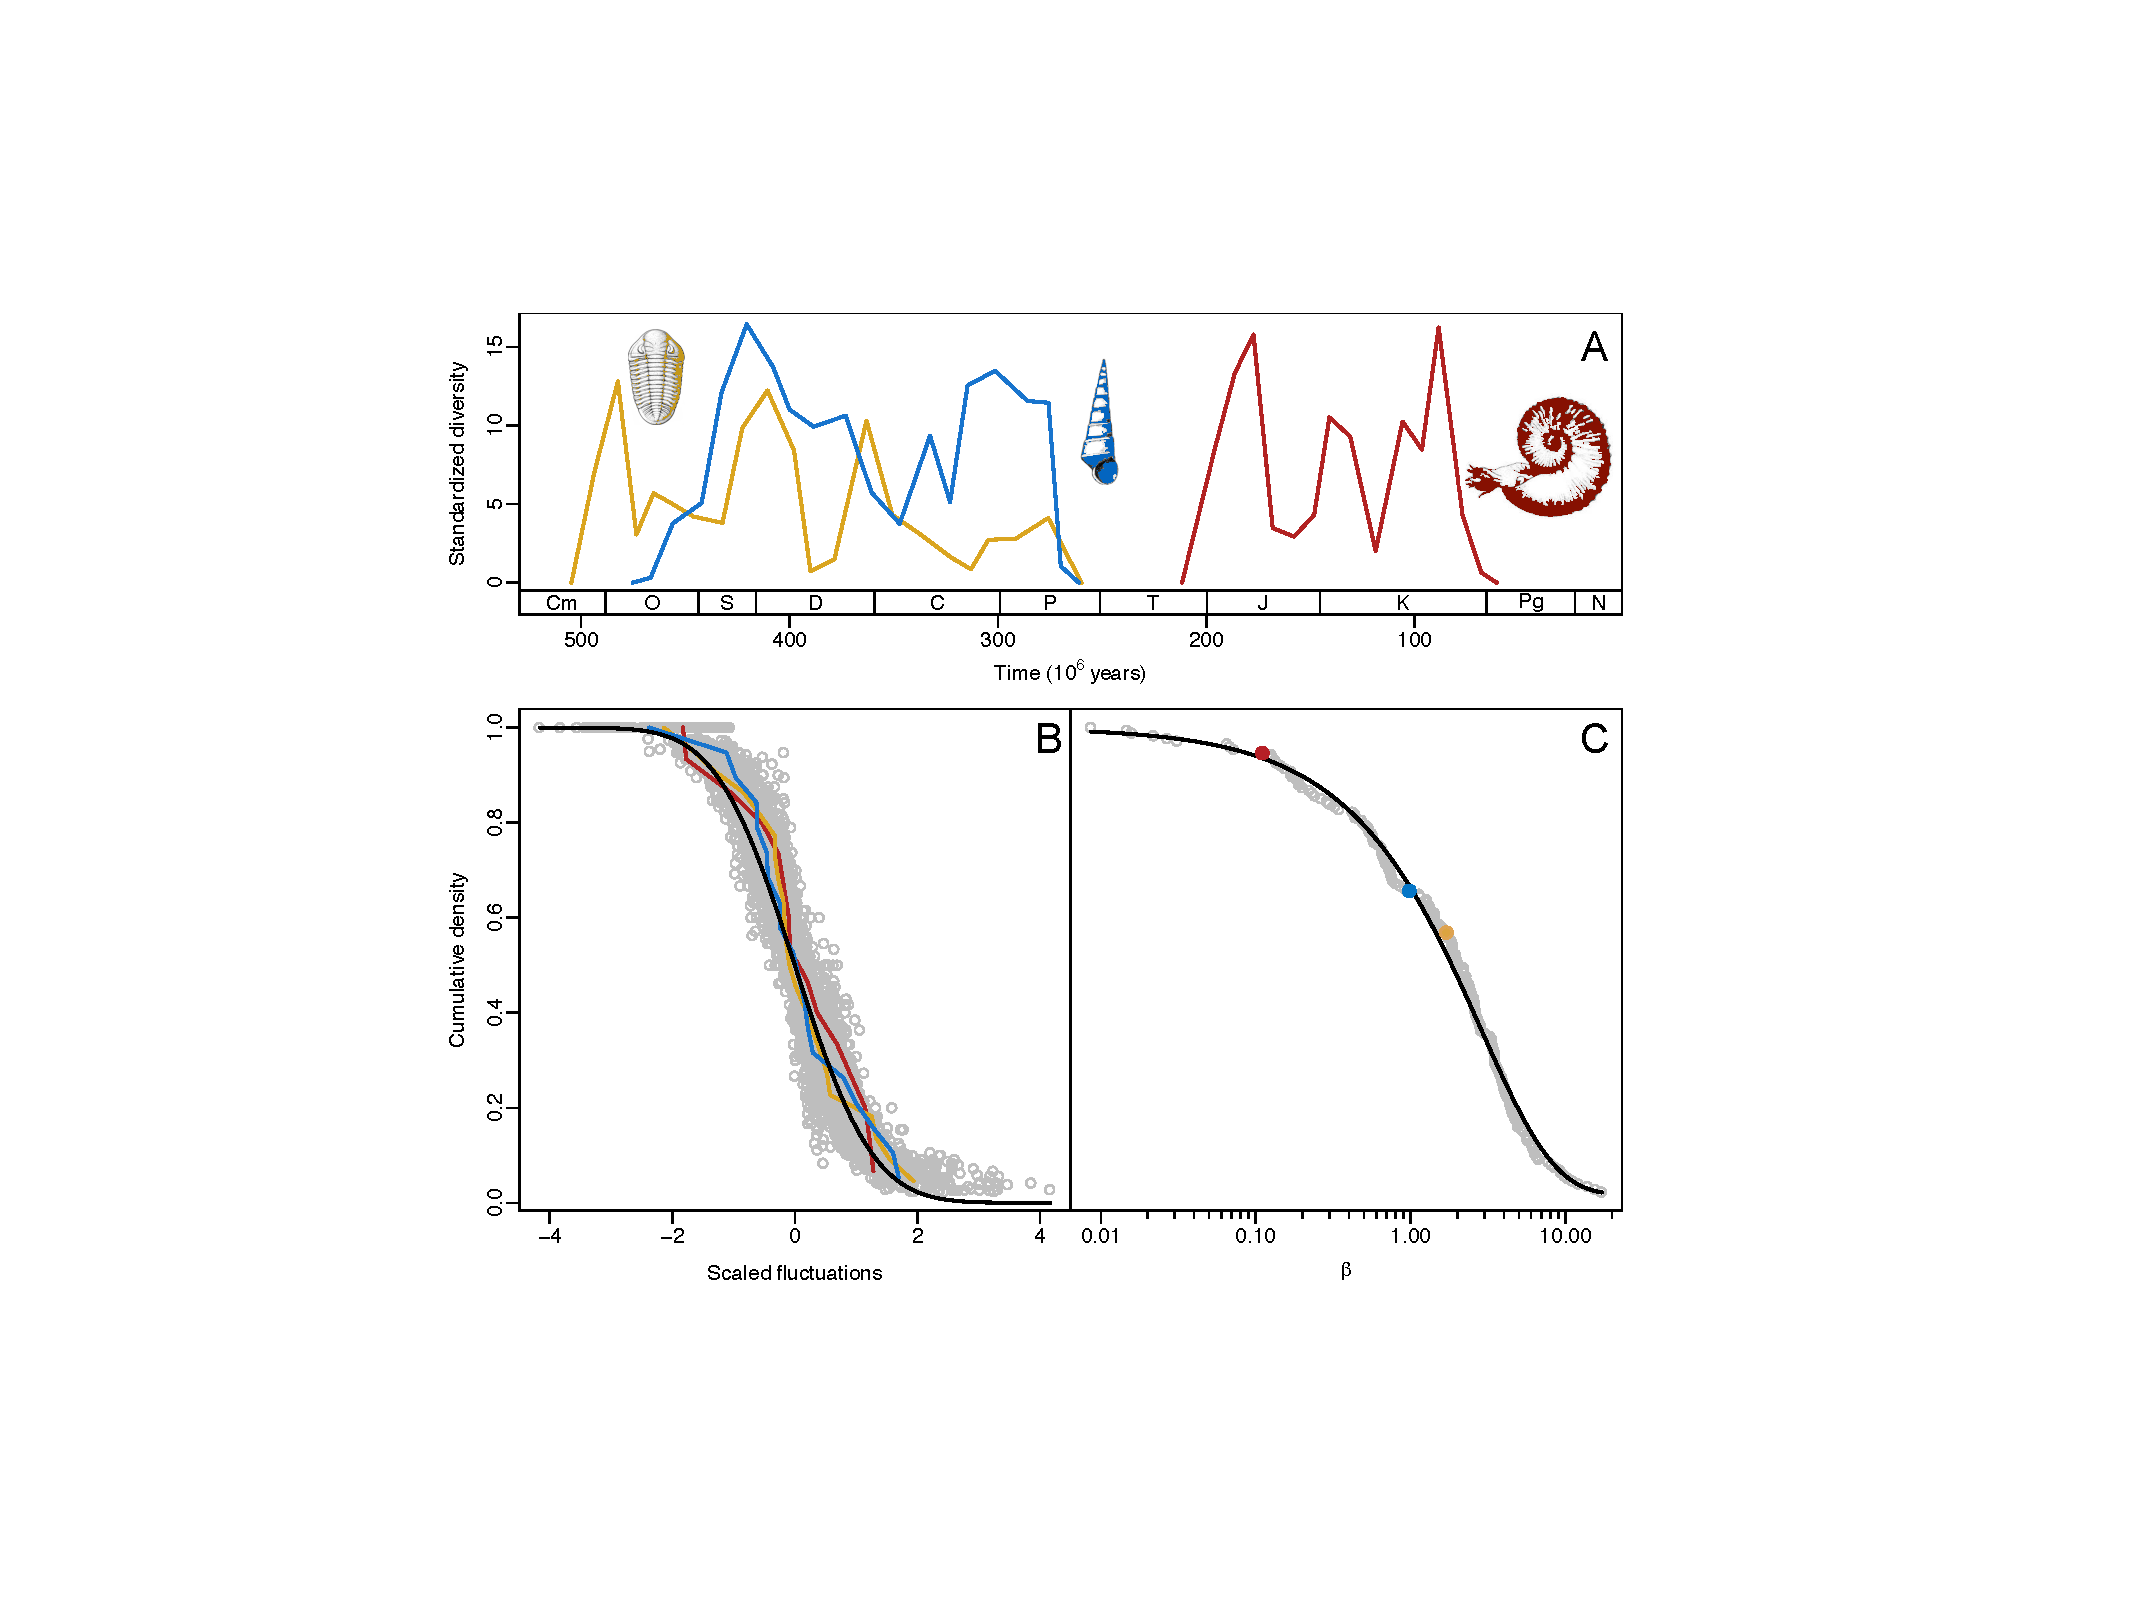
\includegraphics[scale=0.8]{figs/fig_pkx-fbeta.pdf}
  \caption[Variability in trajectories of within-order fluctuations in
  genus diversity]{The distributions of within-order fluctuations in
    genus diversity shown for the trajectories of three exemplar
    orders (A) and shown as an empirical cumulative density aggregated
    across all orders (B). To display all orders simultaneously we
    simply collapse their fluctuation distributions by dividing by
    their standard deviations. If orders conform to the Gaussian
    hypothesis their scaled fluctuations should fall along the
    cumulative density line of a normal N(0, 1) distribution, as shown
    in (B). In (C) the distribution of inverse variances $\beta_k$
    across all orders matches very closely to a Gamma distribution
    (black line); exemplar orders are again highlighted.}
  \label{fig:pk_f}
\end{figure}

In independent and dynamically equilibrial dynamics suggested by these
Gaussian fluctuations in genus richness could result from neutral-like
processes \citep{hubbell2001}, where the dynamics of one taxon are
unaffected by those of another, or from dampening mechanisms that
stabilize complex networks of interacting taxa \citep{brose2005}. This
is in direct contrast to the instability hypothesis underlying the
self-organized criticality theory of paleo-biodiversity
\citep{bak1993, sole1997}.

To predict the super-statistical behavior of the entire marine
invertebrate Phanerozoic fauna we must integrate over all possible
local equilibria that each clade could experience. The stationary
distribution of $\beta_k$ values describes these possible equilibria,
specifying the probability that a given clade, chosen at random, will
occupy a region of niche space characterized $\beta_k$. The form of
this stationary distribution could shed interesting light on the
biological processes that lead different clades to explore different
regions of adaptive landscapes, and thus different equilibria, as
discussed below.

We estimate the distribution of $\beta_k$'s simply as the maximum
likelihood distribution describing the set of inverse variances for
all orders. In both the PBDB and Sepkoski's compendium, Phanerozoic
marine invertebrate orders clearly follow a Gamma distribution in
their $\beta_k$ values (Fig. \ref{fig:pk_f}).  

Using the observation of within order statistical equilibrium and
Gamma-distributed $\beta_k$ parameters we can calculate, without
further adjusting free parameters, the distributions of order-level
fluctuations for the entire marine Phanerozoic, $P(x)$, as
\begin{equation}
  P(x) = \int_0^\infty p_k(x \mid \beta) f(\beta) d\beta \label{eq:PxInt}
\end{equation}
where $p_k(x \mid \beta)$ is the distribution of fluctuations within
an order and $f(\beta)$ is the stationary distribution of inverse
variance in the magnitude of order-level fluctuations in
diversity. This leads to a non-Gaussian, fat-tailed prediction for
$P(x)$ which matches both the PBDB and Sepkoski data closely
(Fig. \ref{fig:Px} and Appendix \ref{sec:suppSepk}).

\begin{figure}[!h]
  \centering
  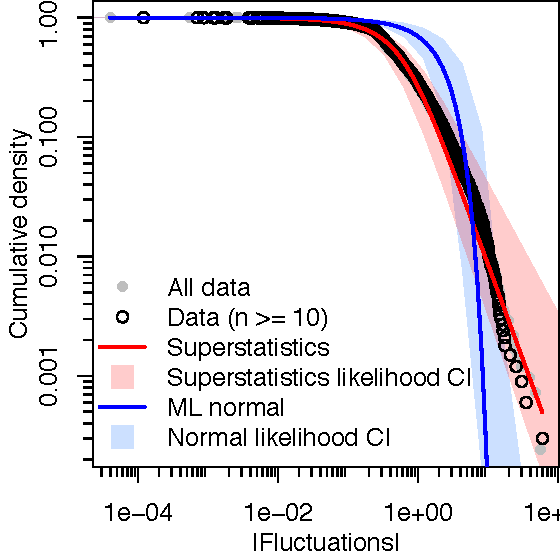
\includegraphics[scale=1]{figs/fig_Px.pdf} 
  \caption[Order-level distribution of diversity
  fluctuations]{Distribution of fluctuations in genus diversity within
    orders of marine invertebrates in the Paleobiology Database
    \citep{alroy08} after bias correction. The distribution is
    fat-tailed as compared to the maximum likelihood estimate of the
    normal distribution (blue line).  At the order level the empirical
    distribution of fluctuations are well described by our
    super-statistical approach, both when computed from integrating
    over the distribution of observed variances (red line) and when
    fit via maximum likelihood (95\% confidence interval; red
    shading).}
  \label{fig:Px}
\end{figure}

To quantitatively evaluate how well the super-statistical prediction
matches the data we constructed a 95\% confidence envelope from
bootstrapped maximum likelihood estimates for $P(x)$. Observed
fluctuations fall within this 95\% confidence envelope
(Fig. \ref{fig:Px}), indicating that the data do not reject the
super-statistical prediction. For further comparison, we fit a
Gaussian distribution to the observed fluctuations, which corresponds
to the equilibrium hypothesis that all orders conform to the same
statistic. Using Akaike Information Criterion (AIC) we find that
observed fluctuations are considerably better explained by the
super-statistical prediction than by the Gaussian hypothesis ({\small
  $\Delta$}AIC = 11285.18). Thus, as expected under the
superstatitical hypothesis, the fat tailed distribution of
fluctuations arise from the superposition of independent Gaussian
statistics of fluctuations within orders.

%% calculating sstat at different taxonomic levels (D-stat fig)
Computing the distribution of fluctuations using classes instead of
orders leads to a substantially poorer fit to the observed data
(Fig. \ref{fig:supp_PBDB_Px_cls}). We quantify this shift with the
Kolmogorov-Smirnov statistic, which changes from 0.041 for orders to
0.062 for classes (Fig. \ref{fig:dStat}). However, if
super-statistical theory explains the data, this worsening fit with
increasing taxonomic scale is expected as the different classes should
not represent dynamically equilibrial sub-systems in their fluctuation
dynamics. Instead, classes aggregate increasingly disparate groups of
organisms, and thus effectively mix their associated Gaussian
fluctuations, meaning that one statistic should no longer be
sufficient to describe class-level dynamics. Our analysis indicates
that orders are evolutionarily equilibrial and independent entities,
with all subsumed taxa sharing key ecological and evolutionary
attributes allowing them to read steady state diversification
independently from other orders. Both the good fit at the order level
and worsening fit at higher taxonomic levels is confirmed in
Sepkoski's compendium, which also allows analysis of phylum-level
patterns (Fig. \ref{fig:supp_sepkPx}).

\begin{figure}[!h]
  \centering
  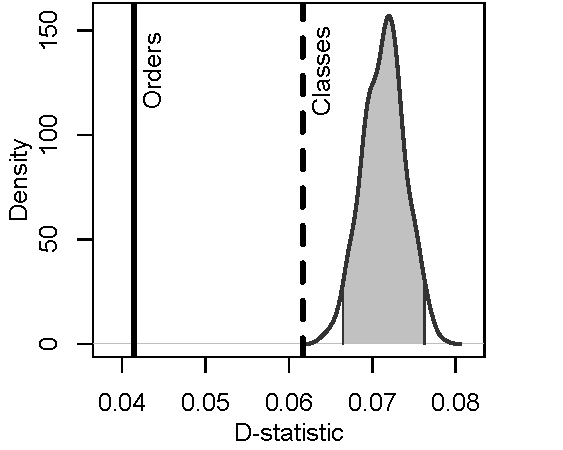
\includegraphics[scale=1]{figs/fig_dStat(3TP).pdf}
  \caption[Goodness of super-statistical theory fit]{Distribution of
    Kolmogorov-Smirnov (KS) statistics from randomly permuting genera
    within orders (gray shading represents 95\% confidence
    interval). Solid black line is observed KS statistic at the order
    level, while the dashed black line shows the observed KS statistic
    at the class level.}
  \label{fig:dStat}
\end{figure}

To further test the evolutionary coherence of orders we conducted a
permutation experiment in which genera were randomly reassigned to
orders while maintaining the number of genera in each order. For each
permutation, we calculated the super-statistical prediction and the
Kolmogorov-Smirnov statistic. The permutation simulates a null model
in which common evolutionary history is stripped away (genera are
placed in random orders) but the total number of observed genera per
order is held constant.  Repeating this permutation 500 times yields a
null distribution of Kolmogorov-Smirnov statistics that is far
separated from the observed value (Fig. \ref{fig:dStat}) suggesting
the good fit at the order level is not merely a statistical artifact
of classification but carries important biological information.

\section*{Discussion}

%% why orders
Our analysis makes no assumption that orders should correspond to
super-statistical subsystems, but identifies them as the appropriate
level for marine invertebrates. Holman \citep{holman1989} has also
shown that orders are ``evolutionarily coherent'' in that subtaxa
within orders share common diversification dynamics. As we show,
orders differ only in the variances of their diversity fluctuations
(Fig. \ref{fig:pk_f}).

Our study is the first to demonstrate that complex patterns in the
fluctuation of diversity resulting from the sequence of origination
and extinction events in the fossil record are the result of a simple
underlying process analogous to the statistical mechanisms by which
complexity emerges in large, non-equilibrium physical \citep{beck2004}
and social systems \citep{fuentes2009}.  We do so by identifying the
biological scale at which clades conform to locally independent
dynamic equilibria in fluctuations. This scale is determined by the
process of niche conservatism \citep{roy2009range, hopkins2014} within
orders.  Equilibrium could result from many processes, including
neutrality \citep{macWilson, hubbell2001}, diversity-dependence
\citep{gavrilets2005, rabosky2009ecolLett} and processes that
dampen---rather than exacerbate---fluctuations in complex ecological
networks \citep{berlow2009}. We then show that punctuated shifts to
different equilibria between order, a consequence of punctuated
exploration of niche space by newly evolving clades
\citep{eldredgeGould1972, newman1985adaptive, hopkins2014}, leads to a
characteristically non-equilibrial distribution of diversity
fluctuations when the marine Phanerozoic fauna is viewed as a whole
macro-system.

The stationary distribution describing this process of punctuated
non-equilibrium is clearly Gamma.  A Gamma distribution, while
consistent with multiple processes \citep[e.g.][]{cir1985}, could
result from evolution of diversification rates across an adaptive
landscape that promotes niche conservatism and punctuated exploration
of niche space.  Specifically, if $\beta_k$ values are associated with
a clade's physiological and life history traits, and those traits
evolve via Ornstein-Uhlenbeck-like exploration of an adaptive
landscape, the resulting stationary distribution of $\beta_k$ will be
Gamma \citep{cir1985, butler2004}.  For macroevolutionary rates to
vary across an adaptive landscape, this landscape cannot be flat, and
thus niche conservatism punctuated by adaptive exploration is
inevitable \citep{newman1985adaptive}. However, if somehow rate
variation could occur in a less peaky landscape, we would expect the
distribution of $\beta_k$ to follow a chi-squared distribution.

%%% how this motivates future work in figuring out the details of
%%% biotic evolution that are important for driving stasis and
%%% punctuation
Our work highlights the importance of both niche conservatism and
punctuated adaptive radiation in producing the statistical behavior of
the Phanerozoic; our theory thus provides new motivation for
identifying the eco-evolutionary causes of innovations between
lineages and how those innovations are eventually conserved within
lineages. Armed with an understanding of the statistical behavior of
diversification we can go on to examine mechanisms underlying
additional patterns in the mean trend of biodiversity through the
Phanerozoic. In particular, clades have been shown to wax and wane
systematically through time \citep{liow2007,
  quental2013}, a pattern that we cannot explain with super-statistics
alone.

%% note on how sstat could be applied to other questions in eco-evo.
Superstatistics could also be applied to other areas of evolution and
macroecology.  For example new phylogenetic models already consider
heterogeneous rates of diversification
\citep[e.g.][]{rabosky2006laser}. The superstatistics of clades in
adaptive landscapes could provide a means to build efficient models
that jointly predict morphological change and diversification. This
framework could also provide a new paradigm in modeling the
distributions of diversity, abundance and resource use in non-neutral
communities. Non-neutral models in ecology are criticized for their
over-parameterization \citep{rosindell2011}, yet a persistent
counter argument to neutral theory \citep{hubbell2001} is the
unrealistic assumption of ecological equivalency
\citep{chave2004neutral} and poor prediction of real dynamics
\citep{ricklefs2006neutral}. If ecosystems are viewed as the
super-position of many individualistically evolving clades, each
exploiting the environment differently and thus obeying a different
set of non-equivalent statistics, then diversity dynamics could be
parsimoniously predicted with superstatistics while incorporating real
biological information on ecological differences between taxa.

Superstatistics is a powerful tool to derive macro-scale predictions
from locally fluctuating sub-systems whoes evolution is driven by
interesting, but complex and difficult to model, biological
mechanisms. As such, applications of superstatistics from islands to
populations to clades are ripe for exploration.


\section*{Methods}

\subsection*{Paleobiology Database data download and filtering}
Data were downloaded from the Paleobiology Database (PBDB;
www.pbdb.org) on 28 May 2013. Collections were filtered using the same
approach as Alroy \citep{alroy08} to insure that only well preserved
marine invertebrate occurrences were used in subsequent analysis
resulting in 221202 genus occurrences. These were further filtered to
exclude those occurrences without order-level taxonomy and those
collections with age estimate resolutions outside the 10my default
bins of the PBDB resulting in 189516 occurrences left for analysis. To
avoid basic sampling concerns we excluded the earliest Cambrian and
the Cenozoic.

To focus attention on the variance of fluctuations we center each
clade's fluctuation distribution. Because ``equilibrium'' in the
statistical mechanical sense means a system undergoes coherent,
concerted responses to perturbation the mean trend line is of less
interest than deviations from it. We also note that most clades are
already close to centered and so centering has little influence on
clade-specific fluctuation distributions.

\subsection*{Three-timer and publication bias correction} 
\label{sec:3TP}
We use a new and flexible method, described below, to correct for
known sampling biases in publication-based specimen databases
\citep{alroy08, alroy2010}.  We were motivated to use this method
because rarefaction has been shown to under-perform compared to the
more data-intensive shareholder quorum subsampling (SQS) method
\citep{alroy2010}.  However, subsampling cannot be applied to small
orders (i.e. the majority) because SQS becomes increasingly unreliable
as sample size decreases \citep{alroy2010}.  We therefore develop a
simple method based on first correcting for detection bias using the
``three timer'' correction \citep{alroy08} in which the rate of failure
to observe a genus is estimated by the number of times a gap occurs in
the occurrence history of each genus. To eliminate further bias due to
preferential publication of novel taxa we divide observed number of
genera per order per time period by the expected number of genera
given publications in that time period.  The expected number is
calculated by regressing the log-transformed number of genera on
log-transformed number of publications. There is a weak trend toward
higher diversity with more publications (Fig. \ref{fig:divByPub})
meaning that the most important correction comes from the three timer
correction.

Our new method effectively re-scales each genus occurrence from 0/1
(absent/present), to a weighted number continuously ranging between 0
and 1.  This method achieves similar results to more computationally
intensive sub-sampling procedures \citep{alroy08, alroy2010}. We
directly compare our predicted time series of global genus diversity
with results derived from SQS \citep{alroy2010} and the raw data
(Fig. \ref{fig:supp_3TPub}).  Our method shows minor differences with
the SQS prediction, However, these discrepancies do not have impact
the distribution of fluctuations (Fig. \ref{fig:supp_3TPub}) and
super-statistical analysis on uncorrected PBDB data (see section
\ref{sec:rawPBDB}) produces a similar result to the analysis on
corrected PBDB data presented in the main text.

\subsection*{Numerical methods} \label{sec:numMeth} To fit our
super-statistical prediction we use the method of least squares
instead and maximum likelihood. When building the prediction for
$P(x)$ by calculating order-level Gaussian distributions and
integrating over them, we use least squares to fit the variance term
to each order. We do so because orders potentially show asymmetries in
their distribution of fluctuations. Least squares is more flexible in
fitting such distributions compared to maximum likelihood which will
always estimate the empirical variance as the best-fitting parameters.

We also estimate $P(x)$ directly from the raw data using maximum
likelihood to compare the fit of our super-statistical prediction and
that of a simple Gaussian distribution using AIC. To calculate a
likelihood-based confidence interval on our prediction we bootstrapped
the data, subsampling fluctuations with replacement from all orders
combined.

\bibliographystyle{Science}
\bibliography{../superStat}


\section*{Acknowledgments}
We thank John Harte, Rosemary Gillespie, Linden Schneider, and Jun
Ying Lim for helpful discussion. We thank the many contributors to the
Paleobiology Database for making data availible, and Michael Foote
provided a digitized copy of Sepkoski's compendium. AJR thanks funding
from Fulbright Chile, the National Science Foundation Graduate
Research Fellowship Program and the Omidyar Program at the Santa Fe
Institute; MAF thanks FONDECYT 1140278; PM thanks CONICYT PFB-023,
ICM-P05-002 and FONDECYT 1161023.


\end{document}

